%% Basic documentation
%%
%% (c) Thomas Hesse
%%
%% folder: ./content/

\chapter{Introduction}
\label{chap:0}

People nowadays can hardly imagine their life without driving. And it is natural since traveling brings independence and freedom to human life. For example, an average American person makes $2.2$ driving trips per day and spends $50.6$ minutes on the road, which makes over $300$ hours every year people spend in their cars \cite{americanDriving}. Despite the joy driving brings to people, traffic safety is a major aspect which cannot be ignored. With increasing time which people spend on the cars, a number of a vehicle-related accident is far away from being perfect. The \gls{WHO} annually announce a report which includes a total number of people lives which were taken away due to car accidents. The latest report was published in December of $2018$ and stated that during this year there was more than $1.35$ million death worldwide \cite{WHOstatistics}. \\
Recent years were full of massive developments towards autonomous driving in autonomous industry. Achievements in one area can be helpful in developing other areas, i.e. great success in image recognition and perception can allow computers to achieve super-human performance \cite{SuperComputer}, etc. Unfortunately, image recognition and environmental perception alone are not enough to solve all the problems of autonomous cars. In ideal circumstances achieving full autonomy of the cars would help not only to save the environment, as well it would benefit traffic participants with more smoothly traffic and more safety on the roads. Industrial innovation experts from ARK Invest strongly believe that with fully autonomous cars accidents on the road would drop to $80$\% \cite{ARKInvest}.\\
Although autonomous cars are something that engaging a wide range of engineers for some time already, this area not fully developed yet and will continue engage engineers even more in the future. At the moment big achievement which is equipped into the majority of new cars is \gls{ADAS}, which for the fact does not enable yet full autonomy of the cars, but it successfully assists driver while driving a car.\\
It is not a secret that all drivers need to interact with each other non-stop in one way or another while they are driving. This communication together with the individual behaviour of a driver is the main key to traffic safety. The behaviour of the driver can be considered as a combination of current traffic observations, short future forecast, decision making and completing actions. The driver should make decisions and actions with full safety concept for himself and other traffic participants. The same is with fully autonomous vehicles: algorithm which is running while a car is driving should ensure all passengers in the car and other traffic participants safety while making decisions and maneuvering through traffic. It is not hard to understand that one of the biggest problem with both the \gls{ADAS} systems and the full autonomous cars is the human factor. To improve \gls{ADAS} systems and achieve safety in fully autonomous cars, prediction methods are essential. Requirements for prediction are precision preciseness (with some time in advance), efficiency and reliability. This thesis will focus on the movement and intention prediction of humans in other cars.

\begin{figure}[h]
	\centering  	
	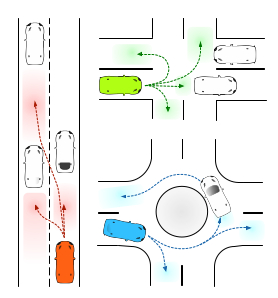
\includegraphics[width=5cm]{img/4.jpg}
	\caption{Insertion Areas (Colored Regions) Under Different Driving Scenarios \cite{pic}}
	\label{fig:intersectionAreas}    
\end{figure}

\section{Background}

Beyond trendy names like Tesla, Google, Aptiv, etc., chasing driverless cars, beyond a large number of automobile brands and other tech engineers, \gls{TuD} has its own \gls{aDDa} working group \cite{aDDa}. \gls{aDDa} initiative started \textcolor{red}{on October 2017}. A group of students and their supervisors from eight different departments at \gls{TuD} are working for one purpose to develop fully autonomous car by themselves, here, at University. All participants of the working group closely cooperate bringing together interdisciplinary know-how experience to jointly set up and operate an autonomous vehicle. One special feature of \gls{aDDa} is that the main work is done in the context of student projects (final thesis, semester work, permanent work at the team, etc.). By working together on the complex tasks of autonomous driving, participants are solving problems for tomorrow. \\
In not so long period of gls{aDDa} existing, it is made a lot of developments and improvement of existing systems. Some works to mention: "Development and Implementation of a Long-Term Dynamics Control for Automated Driving", "Collision Avoidance in Uncertain Environments for Autonomous Vehicles using POMDPs", "Conception and Design of a Camera Mounting and Calibration for Test Vehicle", "Development of an IT Security Concept for an Automated Vehicle, Pedestrian Detection", "Tracking and Intention Prediction in the Context of Autonomous Driving" and much more \textcolor{red}{\cite{aDDa}}. This thesis is also a part of \gls{aDDa} project.

\section{Purpose}

Humans are very irrational and unpredictable and because of that, it is very hard to model them. Moreover, there are no two exact same people, what makes the task to model human behavior almost impossible, since every possible scenario as an endless possible outcome. When an individual is driving it is nearly always necessary to take into account surrounding cars and other traffic participants due to ensure safe, fast and energy optimized journey. \\
Due to the irrationality of humans and recent success and a still big interest in autonomous cars, the purpose of this thesis is to provide an initial step in a probabilistic collision prediction and decision-making system which aims at producing a risk field for the vehicle that predicts
upcoming risks. This step will include creating an algorithm which will use a probabilistic approach and tries to predict future movement and intention of surrounding cars in urban areas.\textcolor{red}{change pictures and maybe explain more about thesis approach in general}.\\
The overall research question is defined
as:
\begin{itemize}
	\item How can probabilistic movement prediction using future estimations be applied for an autonomous vehicle?
\end{itemize}
This research question is then subdivided into smaller questions and task to achieve during in this research work. \textcolor{red}{Three} of these tasks, which are the focus of this thesis, are defined as
\begin{itemize}
	\item Find/create a probabilistic model that learns from various demonstrations. And use this model for trajectory and intention prediction of the car in front of ego vehicle.
	\item Investigate if prior information about environment can improve quality of predictions.
	\item Investigate, how feasible is a probabilistic future movement estimation system, in terms of accuracy and computational time, for real-time applications?
\end{itemize}

\begin{figure}[h]
	\centering  	
	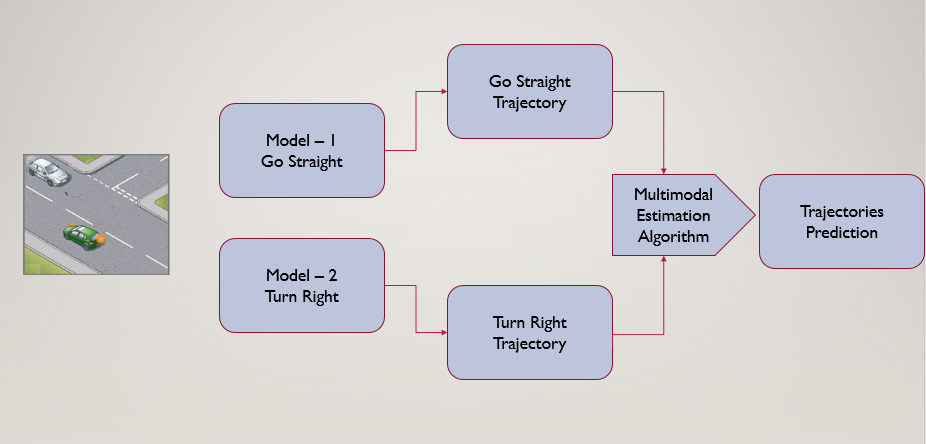
\includegraphics[width=7cm]{img/3.jpg}
	\caption{Scheme of Simple Model Based Approach \cite{pic2}}
	\label{fig:ModBasedApp}    
\end{figure}

The most important thing in driving independent of the car is driverless or need a driver is safety. Safety is not possible without security, and considering this, this thesis will provide an overview of the main security and privacy issues on autonomous driving considering movement prediction. Which leads us to the forth and the final research question for this thesis:
\begin{itemize}
	\item \textcolor{red}{FINALLY DECIDE} 
\end{itemize}

\subsection{Scope of the Thesis}

Autonomous systems are very complex by its' nature and it is natural to make substantial limitations to obtain a reasonable scope for a master’s thesis. This thesis has been decided to use \gls{ROS} environment system, RViz as its' simulation visualization tool, programming part is done in Python and C++ programming languages. Additionally, the evaluated scenarios have been chosen to be T-intersections and crossroads (four-way intersection) with a known environment, limited to only include a single vehicle in addition to the ego vehicle. This choice has been made due to the system complexity, concerning interactions, that multiple cars would introduce. The vehicles in these scenarios are considered to be cars. \\
Furthermore, some research areas which include image processing, object tracking, mapping and trajectory planning will not be addressed since these areas constitute research areas single-handedly. Incorporating any of these areas would make this thesis even more complex and remove attention from what should be the main focus of the thesis: the probabilistic future movement estimation.

\section{Thesis Outline}

This study focuses on developing and evaluating probabilistic based movement and intention prediction algorithm. This
the algorithm uses external cues to predict surrounding vehicles movement in urban situation. \\
The thesis is organized as follows:
\begin{itemize}
	\item Chapter 2. \textbf{Fundamentals and Related works} focuses foundation of the work and presents a theory behind the scope of the thesis.
	\item Chapter 3. \textbf{Approach} describes approaches of the thesis.
	\item Chapter 4. \textbf{Simulation Setup} defines how and why simulation was set in the way in was. Defines inputs for the system and experiments.
	\item Chapter 5. \textbf{Experiments and Results} describes experiments done during the thesis writing period and evaluate results which were received by performing various experiments.
	\item Chapter 6. \textbf{Security Aspects} is based on the fact that "there is no safety without security" and tries to explain the main security and privacy issues of autonomous cars related to movement predictions.
	\item Chapter 7. \textbf{Conclusion and Future Works} wind up this thesis with conclusions and future works based on the findings of previous chapters.
\end{itemize}